% Case-B rotational-stiffness comparison. Entry-angle ranges are the achieved
% pose-based conditions across the three stiffness settings.
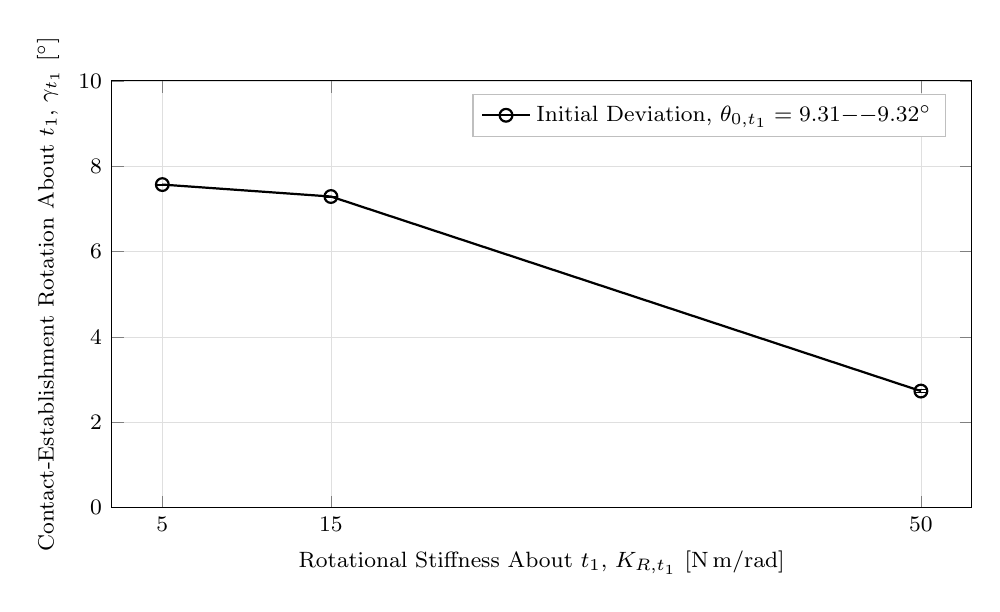
\begin{tikzpicture}
\begin{axis}[
    width=12.5cm, height=7.0cm,
    xmin=2, xmax=53, ymin=0, ymax=10,
    xtick={5,15,50},
    ytick={0,2,4,6,8,10},
    grid=major,
    grid style={gray!25, very thin},
    tick label style={font=\footnotesize},
    label style={font=\footnotesize},
    xlabel={Rotational Stiffness About \(t_1\), \(K_{R,t_1}\) [N\,m/rad]},
    ylabel={Contact-Establishment Rotation About \(t_1\), \(\gamma_{t_1}\) [\(^\circ\)]},
    legend style={font=\footnotesize, draw=gray!50, fill=white,
                  cells={anchor=west}},
    legend pos=north east,
    every axis plot/.append style={thick, mark size=2.3pt},
  ]
\addplot[black, mark=o, error bars/.cd, y dir=both, y explicit] coordinates {
  (5,7.57) +- (0,0.01) (15,7.29) +- (0,0.01) (50,2.73) +- (0,0.03)};
\addlegendentry{Initial Deviation, \(\theta_{0,t_1}=9.31\text{--}9.32^\circ\)}
\end{axis}
\end{tikzpicture}
